As explained in previous sections, the Ginan repository consist on two main components. The \textit{precise orbit deterination} (POD) component estimates precise satellite position and orbital parameters, while the \textit{parameter estimation algorithm} (PEA) monitor systematic biases asociated with GNSS signals. The Ginan software follows uses the \textit{precise point positioning}(PPP) philosophy for processing of GNSS signals. PPP was originally developed as a GNSS based positioning method for calculating location of autonomous receivers with high levels of accuracy and precision. PPP aims to calculate the end user position by rigorously modelling and/or estimating error sources in GNSS measurements. 
The systematic of errors in GNSS signals can be summarised as: 
\begin{itemize}
	\item Satellite state estimation errors: position, clock offset, hardware biases, antenna effects
	\item Receiver state estimation errors: position, clock offset, hardware biases, antenna effects
	\item Atmospheric effects: ionospheric propagation delay, tropospheric propagation delay
	\item Other (modellable) enviromental effects: Relativistic corrections, phase windup
\end{itemize}

The various components of the Ginan software package are designed to model or estimate these errors as parameters. A diagram illustrating of the way the Ginan components interact to estimate these parameters can be found in figure \ref{fig:PEAnPOD}. In the example illustrated by the figure:
\begin{enumerate}
	\item  The POD in orbit fitting mode is used to calculate an a-priori position and the linearization partials of orbit parameters  
	\item  The PEA, in network mode, estimate orbital parameters from orbit partials
	\item  The POD, use the orbital parameters to estimate and predict precise satellite positions
	\item  The PEA, in network mode, is used to estimate wide-area parameters: satellite clock offsets, satellite hardware bias and atmospheric delays 
	\item  The PEA, in end-user mode, is used to callculate local parameters like receiver position, receiver clock offset and local atmospheric delays 
\end{enumerate}

Other parameters, such as antenna, phase windup and relativistic effects are calcuated from predefined models.   

\begin{figure}
	\centering
	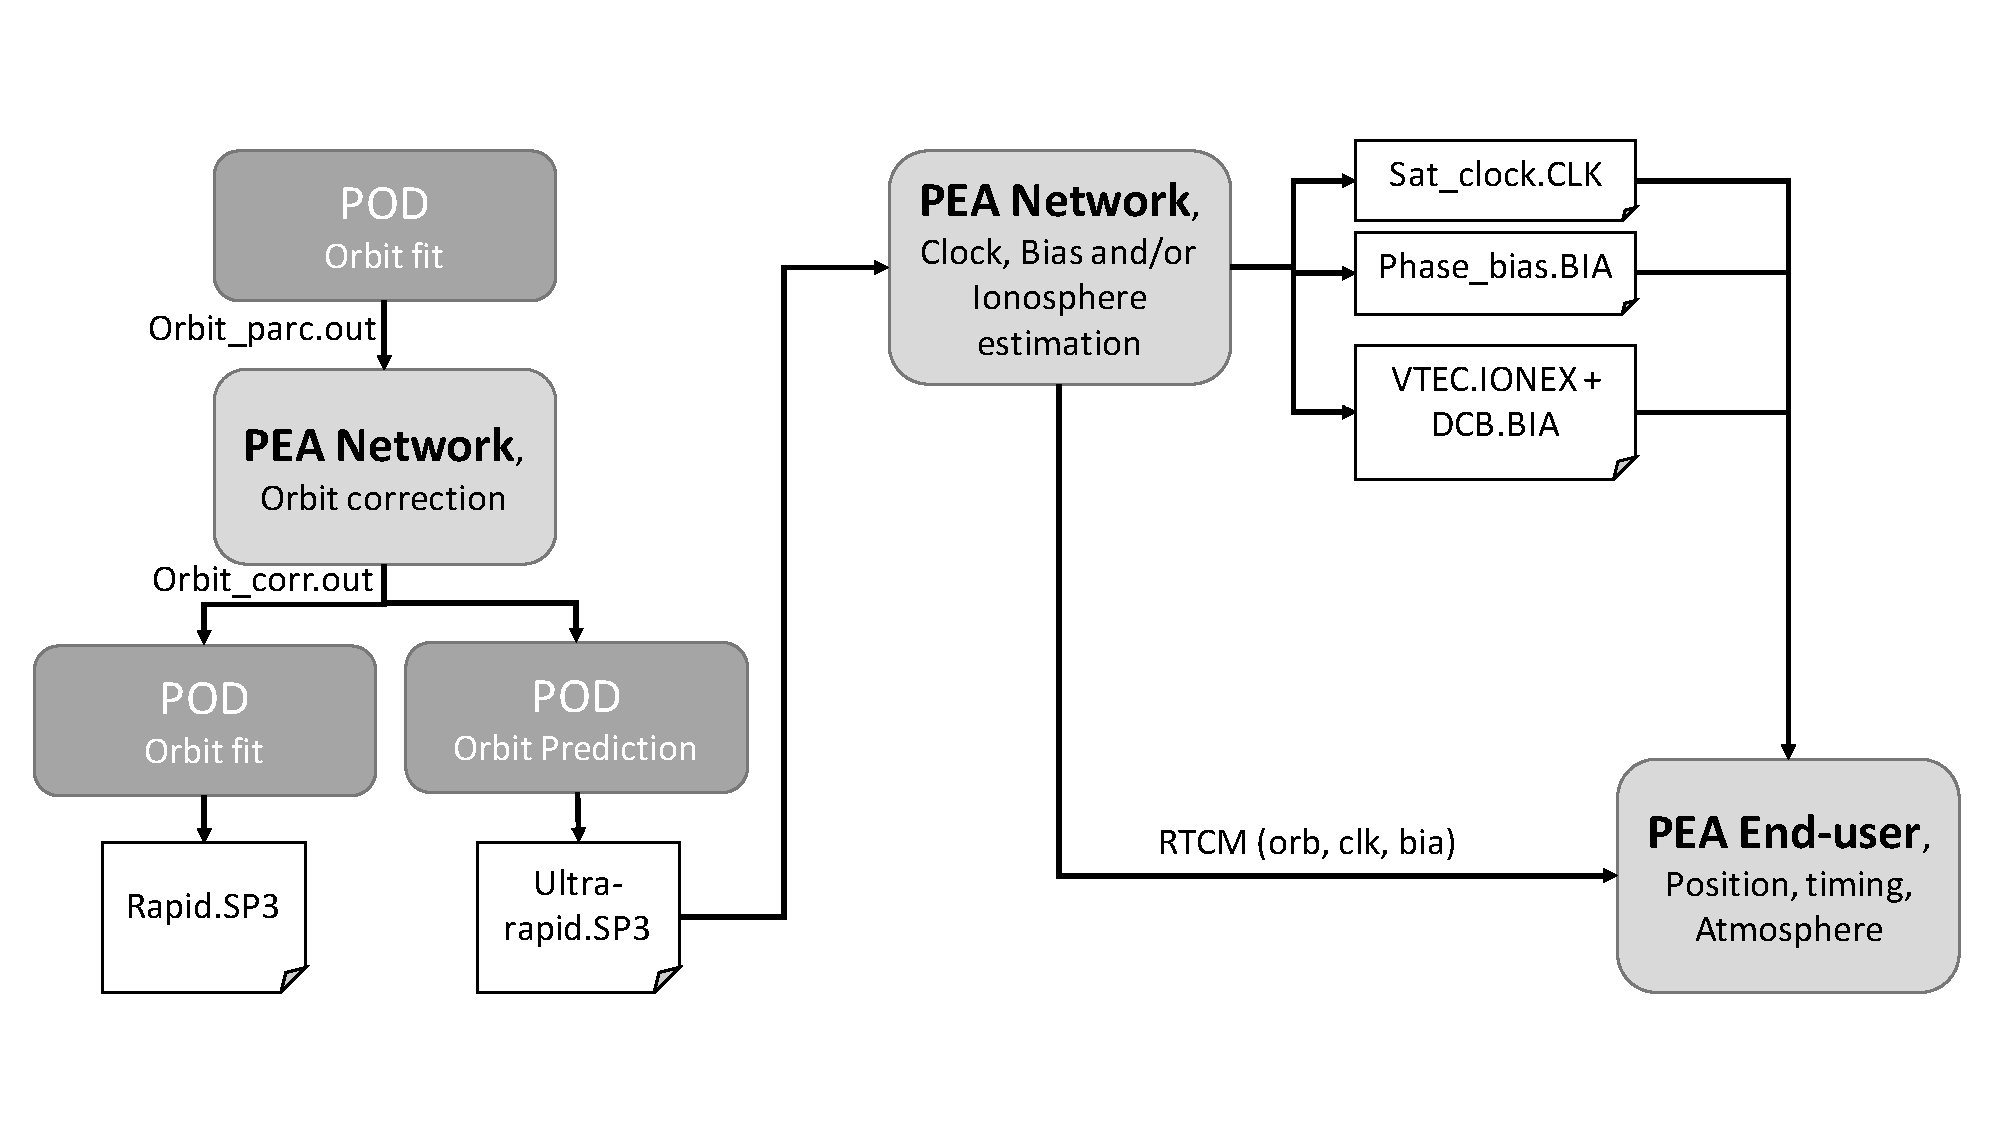
\includegraphics[width=\linewidth]{Ginan_diagram.pdf}
	\caption{Ginan software components}
	\label{fig:PEAnPOD}
\end{figure}

A description of each components and its use is presented below.  \\

\chapter{Using the POD Module}
GINAN applications use YAML format to define configuration files. After installing the dependencies and compiling building the POD application, the POD processing can be started by typing the command.
\begin{verbatim}
$ ./pod -y <path_to_config_file>
\end{verbatim}
Details on the configuration parameters included in YAML files can be found in chapter \ref{ch:pod_yaml_configuration}. Configuration files corresponding to the examples in this section can be found in the \textit{ginan/examples} directory.\\

The POD module has two main modes of operation, the orbit fitting mode and the orbit integration/prediction mode. In orbit fitting mode, precise orbit parameters are calculated from, potentially inaccurate, satellite position pseudo-observations. In orbit integration mode, precise satellite positions are estimated/predicted from precise orbit parameters.\\

\section{Using the POD for orbit fitting}
The orbit fitting mode can be selected by setting the \textit{ pod\_mode\_fit} to true and \textit{ic\_input\_format : sp3} to true. In this mode, the POD will take satellite position pseudo-measurments from a SP3 formatted file and estimate the orbit state of each satellite contained in the SP3 file. The SP3 file containing a priory satellite position needs to be specified as the \textit{pseudobs\_orbit\_filename} parameter.
The orbit state in POD is represented by a set of parameters consisting of 
\begin{itemize}
	\item Satellite position (in ITRF or TCRF) at the first epoch in the SP3 file
	\item Satellite velocity (in ITRF or TCRF) at the first epoch in the SP3 file
	\item Up to 9 parameters describing the Solar Radiation Pressure over the fitting time
\end{itemize}
These initial conditions, and the models described in chapter \ref{ch:observation_modelling} will allow for the precise determination of satellite positions over the fitting arch (set by the \textit{orbit\_arc\_determination} parameter).\\

The main outputs from this mode of operation are the a-posteriori satellite position in SP3 format, and the orbit partials of satellite positions with respect to the initial conditions. 
The ouput SP3 file which can be found on \textit{output\_directory/gagWWWWD.sp3} where \textit{WWWW} is the GPS week and /textit{D} is the GPS day of the first epoc on the SP3 files.
The orbit partials are written in Ginan's proprietary Initial Conditions File (ICF) format, and can be found in  \textit{output\_directory/gagWWWWD\_orbit\_partials.out}.
Configuration files, \textit{ex21\_pod\_fit\_gps} and \textit{ex21\_pod\_fit\_gnss},  for this mode of operation are included in Ginans \textit{examples} folder.\\

\section{using the POD for orbit integration/prediction}
The orbit fitting mode can be selected by setting the \textit{ pod\_mode\_ic\_int} to true and \textit{ic\_input\_format : icf} to true. 
 In this mode, the POD will take the initial conditions contained in the ICF formatted files and propagaes the satellite positions forward over the time period specified by the sum of \textit{orbit\_arc\_determination} and \textit{orbit\_arc\_prediction} parameters. 
 It also propagates the satellite position backwards by a number of hours specified by the \textit{orbit\_arc\_backwards} parameter.
 The ICF file containing the satellites initial condition and radiation pressure parametes needs to be specified as the \textit{ic\_input\_format : ic\_filename} parameter.\\

It is to note that the orbit fitting mode will also use the orbit integration operation after estimating the initial conditions from pseudo-observations. 
Although the  mode \textit{ pod\_mode\_fit} will only integrated for a number of hours specified  by \textit{orbit\_arc\_determination}.
Selecting the \textit{pod\_mode\_predict} will propagate the initial conditions a number of hours specified by the sum of \textit{orbit\_arc\_determination} and \textit{orbit\_arc\_prediction}
The integrated/predicted satellite position will be output to a SP3 formatted file located in \textit{output\_directory/gagWWWWD.sp3}.\\

The configuration file to perform orbit integration/prediction from SP3 files is \textit{ex23\_pod\_prd\_gps}.  
The configuration file to perform orbit integration/prediction from ICF files is \textit{ex24\_pod\_ic\_gps}. Both located in Ginans \textit{examples} folder.\\

